%%%% Marco teórico
%\setcounter{chapter}{1} % para comenzar a partir del capitulo 2

\chapter{FOTOMULTIPLICADORES DE SILICIO}
\label{Cap:MarcoT}
Los fotomultiplicadores de silicio son fotodetectores de estado sólido, comúnmente llamados contadores de fotones, abordan el desafío de la detección y cuantización de señales lumínicas del orden de hasta un fotón \citep{Intro_SIPM_Sensl}. Estos dispositivos han desplazado a los tubos fotomultiplicadores (PMTs) que por mucho tiempo cumplieron esta función \citep{MPPC_note}. Los SiPMs se componen de múltiples pixeles APDs (fotodiodos de avalancha) operando en modo Geiger \citep{Apd_Hamamatsu}. En este capítulo se describe el principio de funcionamiento de los APD y se estudian las características principales de los SiPMs.
% \section{Semiconductores}
% Los materiales semiconductores se encuentran en los grupos tres al cinco de la tabla periódica; es decir tienen entre tres y cinco electrones de valencia, siendo el silicio el más comúnmente utilizado en microelectrónica y en detectores semiconductores. La estructura atómica de los semiconductores es periódica y forma lo que se conoce como una red cristalina en la que los átomos forman enlaces covalentes. A temperaturas por debajo de los 50 K los electrones compartidos en los enlaces covalentes permanecen ligados y el material se comporta como aislante. A temperaturas superiores a 50 K se pueden romper los enlaces debido a vibraciones en la red, permitiendo que algunos electrones se liberen \citep{Detectores_silicio}. En este sentido, como consecuencia de los enlaces covalentes rotos se genera lo que se denomina par electrón hueco, estas partículas tienen la misma carga, pero con signo contrario y pueden moverse por la influencia de un campo eléctrico en direcciones opuestas. Así, Cuando el número de electrones y huecos es igual se tiene un semiconductor intrínseco; el caso contrario se genera por impurezas comúnmente agregadas intencionalmente para aportar electrones (tipo n) o agregar huecos (tipo p).\\ 
% Desde la teoría de bandas se puede explicar las propiedades eléctricas de los materiales. Entre la banda de valencia y la banda de conducción existe una banda prohibida (gap), esta banda no puede ser ocupada por los electrones y su ancho de energía determina si el material es conductor, semiconductor o aislante, como se muestra en la fig. \ref{fig:bandas}.   
% \begin{figure}[h!]
%     \begin{centering}
%         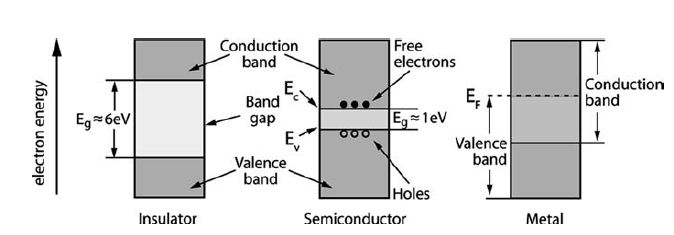
\includegraphics[scale=0.7]{Images/band_energy.JPG}
%         \caption{Estructura de las bandas de energía para aislantes, semiconductores y metales. Adaptado de \citep{Tavenier_Book}.}
%         \label{fig:bandas}
%     \par\end{centering}
% \end{figure}
%\section{El telescopio de muones (MuTe)}
\section{UNIÓN PN}
Es la estructura fundamental de los dispositivos semiconductores, su estudio permite comprender el funcionamiento de los SiPMs. Esta unión se forma al combinar en una región un material tipo P con otro tipo N. En la interfaz entre estas secciones se genera un gradiente de concentraciones de huecos y electrones y aparece una corriente de difusión que hace que los electrones de la zona N se desplacen a la zona P y los huecos de la zona P vayan a la zona N. El proceso de esta recombinación en la unión PN genera la llamada zona de deflección y las cargas agrupadas en esta zona generan un campo eléctrico que se opone a la corriente de difusión y hace que la unión entre en equilibrio, como se muestra en la fig. \ref{fig:PNjuntion}.
\begin{figure}[h!]
\begin{centering}
  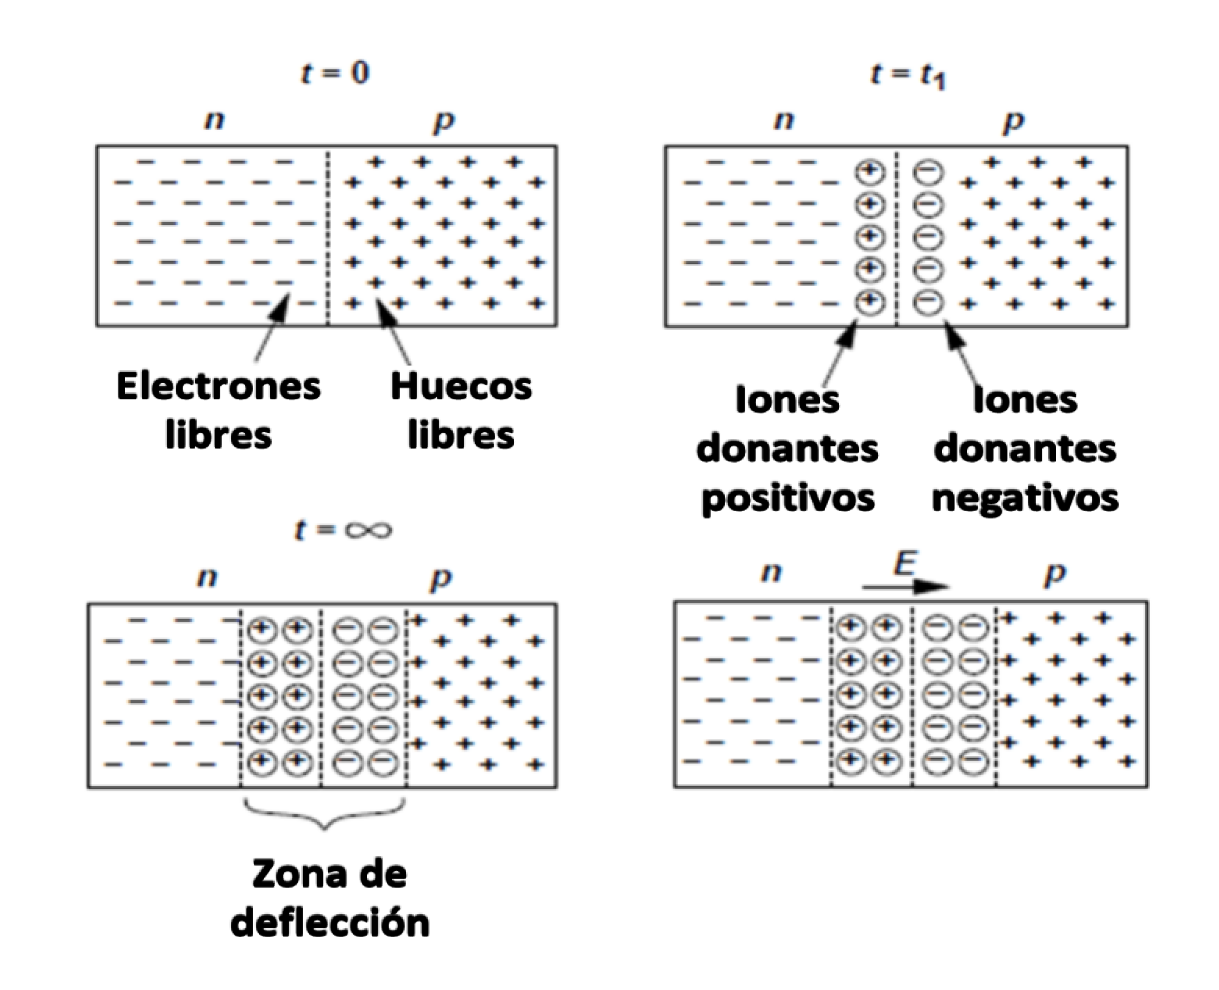
\includegraphics[width=0.5\textwidth]{Images/UnionPN.eps}
  \caption{Evolución de las concentraciones de carga en la unión PN. Adaptado de \citep{Book_razavi}.}
  \label{fig:PNjuntion}
  \par\end{centering}
\end{figure}
\\ \\ 
La diferencia de potencial en la zona de deflección es típicamente de $0.7~$V para el silicio. En polarización directa el voltaje aplicado debe superar los  $0.7~$V para que la región PN entre en conducción. Sin embargo, para una polarización inversa el voltaje aplicado reforzará el campo eléctrico en la zona de deflección, en el caso en que se genere un par electrón-hueco en esta zona, el campo eléctrico le suministra la energía para que se desplace por la unión generando una corriente.\\ \\% sin ninguna amplificación.\\
Existen diferentes formas para que se creen un par de portadores de carga dentro de  la zona de deflección. Por excitación térmica los electrones pueden adquirir la energía necesaria para superar la barrera generada por el dopaje entre la banda de valencia y la banda de conducción. Por otra parte, el efecto túnel, predice una probabilidad que los electrones en la banda de valencia superen la barrera de potencial (band gap) y pasen a la banda de conducción. Esta probabilidad aumenta para altos niveles de voltaje inverso aplicado \citep{tesis_caract_SIPM}. Por último, si la zona de deflección se expone a fotones con energías mayores a la banda prohibida, que para el silicio es de $1.14$ eV \citep{MPPC_note}, se genera un par electrón-hueco debido al efecto fotoeléctrico.\\ \\

% Este  es el principio de funcionamiento de los  fotodiodos PN, una característica que afecta su fotosensitividad y su respuesta en frecuencia es la profundidad de la zona de deflección, que está determinada por:
% \begin{equation}
%   d=\sqrt{\frac{2\varepsilon V_0}{eN}} 
%   \label{depth_PN}
% \end{equation}
% En la ecuación \ref{depth_PN} $\varepsilon$ es la permitividad absoluta, $V_0$ es la diferencia de potencial en la unión PN y $N$ representa la menor de las concentraciones de dopaje entre las uniones P y la N. La capacitancia de un condensador de placas paralelas está dada por:
% \begin{equation}
%   C=\frac{\varepsilon A}{d} 
% \end{equation}
% donde $A$ representa el área de las placas y d es la distancia entre ellas. De las expresiones anteriores se puede obtener la capacitancia por unidad de área como:
% \begin{equation}
%   \frac{C}{A}=\frac{\varepsilon}{d}=\sqrt{\frac{\varepsilon e N}{2 V_0}} 
% \end{equation}
% La expresión anterior es importante porque la capacitancia de la unión representa una fuente de ruido; por ejemplo, el ruido térmico asociado a esta aumenta de forma inversamente proporcional a la capacitancia, sin embargo el ancho de banda se reduce y la respuesta en frecuencia mejora.\\
% Al realizar una polarización inversa de la unión PN se reduce la calidad de la respuesta en frecuencia del fotodiodo, para solucionar esta deficiencia se agrega un semiconductor intrínseco entre las regiones P y N, formando lo que se conoce como fotodiodo PIN, en este fotodiodo la capacitancia en la zona de deflección se reduce con respecto a el fotodiodo PN, lo que genera un incremento en el ancho de banda y hace de este tipo de fotodiodo una buena opción para trabajar con señales de alta frecuencia. Sin embargo, al tener una ganancia unitaria la cantidad de fotones detectados deben ser lo suficientemente grande para generar una corriente eléctrica de una amplitud medible.
% A continuación se estudian un tipo de detectores que tienen una ganancia intrínseca y que se pueden utilizar para la detección de señales lumínicas del orden de un par de fotones.         
\section{ESTRUCTURA GAPD}
Cuando aumenta el voltaje inverso aplicado en la unión PN, también lo hace el campo eléctrico en la región de deflección. Por este motivo, los pares electrón-hueco generados en esta región colisionan con los átomos del material desprendiendo más electrones por ionización de impacto y generando una amplificación de carga mediante una reacción en cadena, conocida como \textit{avalancha}. Los dispositivos que funcionan bajo este principio se llaman fotodiodos de avalancha (APDs) y la corriente que generan es proporcional a la cantidad de fotones incidentes. \\ \\
% \begin{figure}[h!]
% \begin{centering}
%   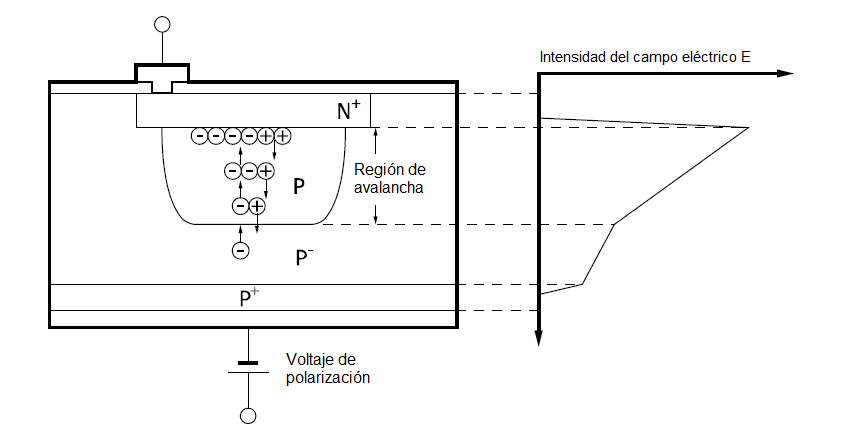
\includegraphics[width=0.7\textwidth]{Images/APD_region.png}
%   \caption{Estructura interna de un APD de silicio. Se muestra la región de avalancha y la intensidad del campo eléctrico en las distintas regiones. Adaptado de \citep{MPPC_note}.}
%   \label{fig:APD_region}
%   \par\end{centering}
% \end{figure}
%El número de pares electrón-hueco generados durante el tiempo que un fotoelectrón recorre una unidad de distancia se denomina tasa de ionización. Normalmente la tasa de ionización de electrones es $\alpha$ y de los huecos es $\beta$. Para el silicio la tasa de ionización de los electrones es mayor que la de los huecos \citep{ionization_rate}. Es por eso que la estructura de los APD mostrada en la fig. \ref{fig:APD_region} se diseña para que los electrones de los pares electrón-hueco generados por los fotones incidentes, entren fácilmente en la región de avalancha\citep{Measuring_ectr_opti_SIPM_hamamatsu}.\\ \\ 
En la figura \ref{fig:APD_gain} se muestra el comportamiento típico de la ganancia en un APD en función del voltaje inverso. En esta gráfica se pueden identificar tres regiones: la primera para voltajes mayores a $50$~V (A); la segunda para voltajes entre $50$ y $100$~V (B) y la tercera para voltajes mayores a $100$~V (C). En la región B la ganancia es lineal con un campo eléctrico moderado, que permite obtener una relación directa entre la entrada (fotones) y la salida (corriente). Sin embargo, en la región C se observa que la ganancia pierde su linealidad y aumenta de forma exponencial cuando se acerca a $150$ V. El voltaje  donde la ganancia tiende a infinito se denomina voltaje de ruptura ($V_{BD}$). En este punto la avalancha generada no puede detenerse así misma, causando que un único fotón genere un pulso Geiger.%quien junto con Walter M\"uller desarrolló el tubo G-M utilizado para la detección de radiación ionizante.\\ \\
\begin{figure}[h!]
\begin{centering}
  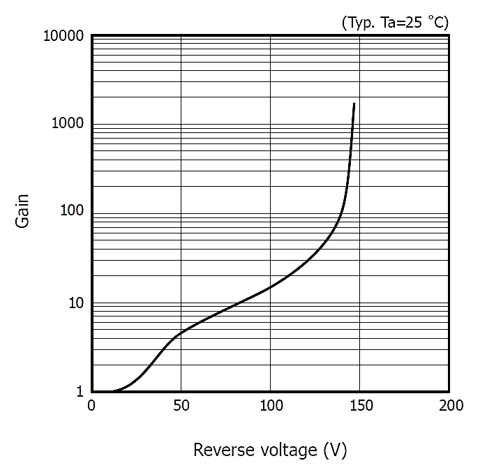
\includegraphics[width=0.5\textwidth]{Images/GAPD_gain.JPG}
  \caption{Ganancia del APD en función del voltaje de polarización inverso donde se pueden observar las regiones de operación del dispositivo. Adaptado de \citep{MPPC_note}.}
  \label{fig:APD_gain}
  \par\end{centering}
\end{figure}
 \\ \\
Un APD operando en modo Geiger se conoce como GAPD. Este dispositivo se caracteriza por tener un elemento externo que permite detener la avalancha y así evitar su destrucción. El procedimiento de apagado se puede realizar utilizando una resistencia que genere una caída de voltaje y reduzca la alimentación del APD, o se puede realizar con elementos activos (\textit{switch}) que permitan desconectar la fuente de alimentación del APD cuando se genere la avalancha.\\ \\
En los GAPD la señal de salida del sensor (amplitud de la avalancha) no es proporcional a la entrada (fotones), por lo tanto a partir de un GAPD no se puede determinar si lo que generó la avalancha fue uno, dos o \textit{n} fotones. La carga generada por la avalancha está determinada únicamente por la ganancia del GAPD que  depende del voltaje de polarización.     
\begin{figure}[h!]
\begin{centering}
  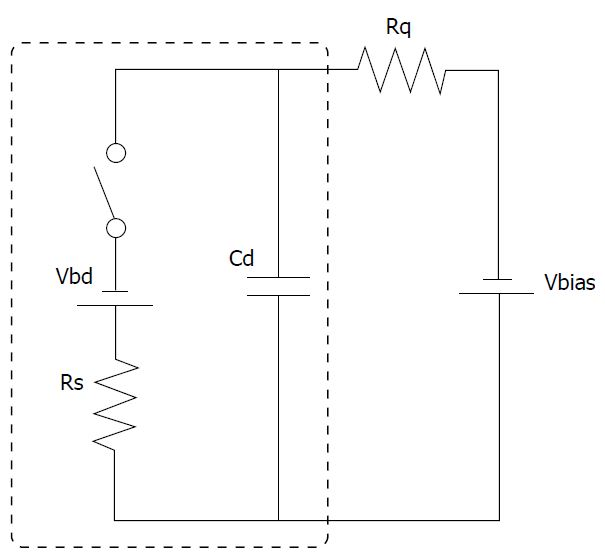
\includegraphics[width=0.5\textwidth]{Images/GAPD_model.JPG}
    \caption{Modelo eléctrico de un GAPD, este modelo corresponde a un circuito RC en serie. La conexión eléctrica típica del GAPD es con una resistencia de apagado y una fuente de polarización en serie.}
    \label{fig:APD_model}
  \par\end{centering}
\end{figure}
\\ \\
El modelo eléctrico  de un GAPD está compuesto por una resistencia en serie con una fuente de voltaje DC (con valor $V_{bd}$) y un interruptor que se cierra cuando el GAPD recibe luz, todo esto en paralelo con la capacitancia de la unión PN, como se muestra en la fig. \ref{fig:APD_model}. En este circuito cuando el interruptor está abierto, $C_d$ se carga por medio de $V_{bias}$, una vez el interruptor se cierra, $C_d$ comienza a descargarse y la corriente del capacitor $I_d$ se bifurca en las dos mallas y su expresión es:
\begin{equation}
    I_d=\frac{V_d-V_{bd}}{R_s}+\frac{V_{bias}-V_d}{R_q},
\end{equation}
donde, $V_d$ es el voltaje en el capacitor, $R_q$ es la resistencia de apagado y $R_s$ representa el comportamiento resistivo del GAPD.
\begin{figure}[h!]
\begin{centering}
  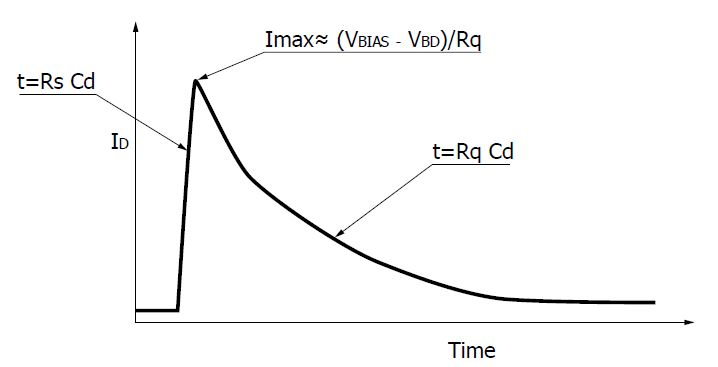
\includegraphics[width=0.6\textwidth]{Images/GAPD_response.JPG}
    \caption{Forma de un pulso de corriente generado por un GAPD. Esta forma típica corresponde a la corriente de carga y descarga de un capacitor en un circuito RC en serie.}
    \label{fig:APD_response}  
  \par\end{centering}
\end{figure}
\\ \\
En la figura \ref{fig:APD_response} se observa la respuesta en el tiempo de $I_d$, esta repuesta está determinada por las contantes de tiempo de carga y descarga  $R_s C_d$ y $R_q C_d$ respectivamente.\\    
\section{EL FOTOMULTIPLICADOR DE SILICIO}
% Los fotomultiplicadores de silicio han tomado cada vez más importancia en aplicaciones científicas e industriales \citep{Blue_SIPM}. Sus usos más conocidos son en los campos de Imágenes médicas \citep{SiPM_PET} , biofotónica \citep{SiPM_bio, SiPM_bio2}, LIDAR \citep{SiPM_Lidar, SiPM_3D_img} y física de altas energías  \citep{Mute_oficial, minimute}. Las principales ventajas de los SiPMs son su alta eficiencia, bajo voltaje de operación, bajo consumo de potencia y robustez mecánica.\\
Como se mencionó en la sección anterior, a partir de un GAPD no se puede determinar el número de fotones que generan un evento o avalancha. Por el contrario, un SiPM sí puede determinar el número de fotones que inciden en el dispositivo, puesto que utiliza una matriz de píxeles, donde cada píxel es un  GAPD en serie con una resistencia de apagado. \\ \\
Como estos píxeles se encuentran conectados en paralelo la respuesta del SiPM es la suma de las avalanchas generadas por cada píxel activado, lo que produce una salida que es directamente proporcional al número de fotones incidentes, siempre y cuando este número no sea superior al número de píxeles con que cuenta el SiPM. El pulso de menor amplitud que se puede observar a la salida de un SiPM es conocido como fotón equivalente (p.e.) y es un parámetro que experimentalmente se utiliza para determinar la ganancia, conteo oscuro, \textit{crosstalk} y \textit{afterpulse} de un SiPM.
\begin{figure}[h!]
\begin{centering}
  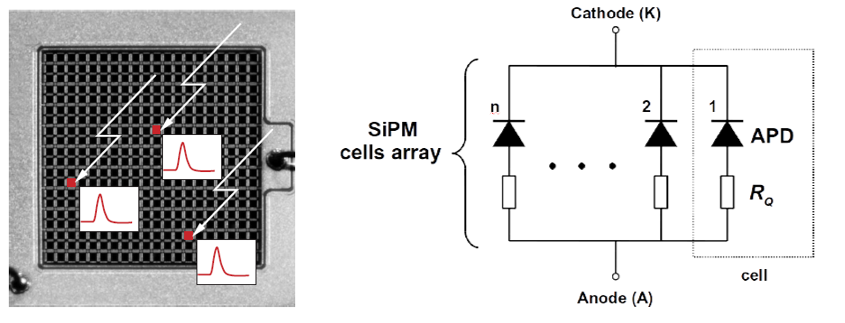
\includegraphics[width=0.75\textwidth]{Images/APD_array.PNG}
    \caption{Estructura de un SiPM, compuesto por microceldas de GAPDs conectadas en paralelo. Adaptado de \citep{Muon_counting_Amiga}.}
    \label{fig:APD_array}  
  \par\end{centering}
\end{figure}
\\ \\
En la figura. \ref{fig:APD_array} se observa la matriz de píxeles de un SiPM, donde cada una de estas microceldas se activan simultáneamente para generar una corriente proporcional a los fotones incidentes. El tamaño de estos píxeles para SiPMs comerciales normalmente es de 25, 50 y 75 $\mu$m, como se muestra en la fig. \ref{fig:APD_pitch}.     
\begin{figure}[h!]
\begin{centering}
  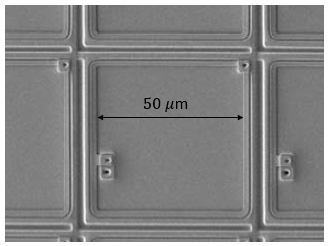
\includegraphics[width=0.5\textwidth]{Images/SiPM_pixel.PNG}
    \caption{Microcelda (píxel) de un SiPM, donde se observa el área fotosensible y la resistencia de apagado al rededor de esta. Adaptado de \citep{MPPC_note}.}
    \label{fig:APD_pitch}  
  \par\end{centering}
\end{figure}

\subsection{Parámetros de rendimiento}
\subsubsection{Sobre-voltaje.}
El voltaje de ruptura es el voltaje mínimo que se necesita para generar el campo eléctrico suficiente en la región de deflexión  para producir la descarga Geiger. Asimismo, la diferencia entre el voltaje de polarización ($\mbox{V}_{Bias}$) y el de ruptura ($\mbox{V}_{BD}$) es lo que se define como sobre-voltaje ($\mbox{V}_{OV}$).
\begin{equation}
V_{OV} = V_{Bias}-V_{BD}.
\label{Vbd_equation}    
\end{equation}
Típicamente, el fabricante suministra el valor de sobre-voltaje al que se debe someter el dispositivo, en el caso del SiPM S13360-1350CS de Hamamatsu el valor es $ 3~\mbox{V}$.
\begin{figure}[h!]
\begin{centering}
  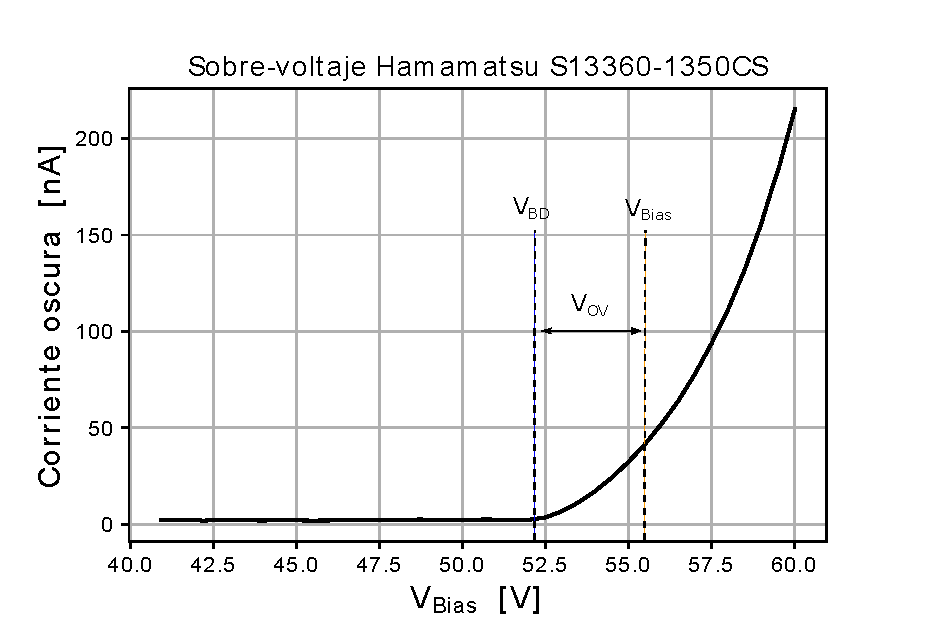
\includegraphics[width=0.7\textwidth]{Images/overvoltaje.eps}
    \caption{Corriente oscura como función del voltaje de polarización a $25~^\circ C$, para el SiPM  S13360-1350CS de Hamamatsu. El sobre-voltaje es la diferencia entre el voltaje de polarización y el voltaje de ruptura.}
    \label{fig:Overvoltage}  
  \par\end{centering}
\end{figure}
\subsubsection{Ganancia.}
La ganancia del SiPM, está definida como la relación entre la carga generada por un pulso Geiger y la carga de un electrón. Así, su valor puede ser calculado experimentalmente a partir un histograma de carga, el cual se caracteriza por tener picos relacionados con el número de fotones equivalentes (p.e.). La distancia entre estos picos es constante  y corresponde a la carga de un pulso  Geiger. La ganancia se define como: %tiene una relación directamente proporcional al sobre voltaje, a la capacitancia y al tamaño de la microcelda.\\
\begin{equation}
    G=\frac{Q_{1p.e.}}{e} = \frac{C\times V_{OV}}{e},
    \label{Gain_eq}
\end{equation}
donde, $Q_{1p.e.}$ es la carga de un fotón equivalente, $C$ es la capacitancia del SiPM, $V_{OV}$ es el sobre-voltaje y \textit{e} es la carga del electrón \citep{Intro_SIPM_Sensl}.
\subsubsection{Eficiencia de detección.}
La eficiencia de detección (PDE, por sus siglas en Inglés) es la probabilidad de que un fotón incidente genere un evento (Pulso Geiger) en alguna de las microceldas del SiPM. En la figura. \ref{fig:PDE}, se muestra la PDE en función de la longitud de onda, en este caso se presenta un pico en su eficiencia para 450 nm. La eficiencia define matemáticamente como:
\begin{equation}
    PDE= FF\times QE \times P_{Trig},
\end{equation}
donde, FF es el factor de llenado y  se define como la relación ente el área sensible y el área inactiva del SiPM, este valor puede  estar entre el 30\% y el 80 \%, en función del tamaño del píxel. Por otra parte, QE es la eficiencia cuántica y expresa la probabilidad que un fotón incidente sea transmitido al silicio y finalmente convertido en un par electrón-hueco \citep{Study_SiPM}. Finalmente, $P_{Trig}$ es la probabilidad que un par electrón-hueco genere una avalancha, este parámetro depende del sobre-voltaje y de la longitud de onda de los fotones incidentes \citep{Study_SiPM_FBK}.\\

\begin{figure}[h!]
\begin{centering}
  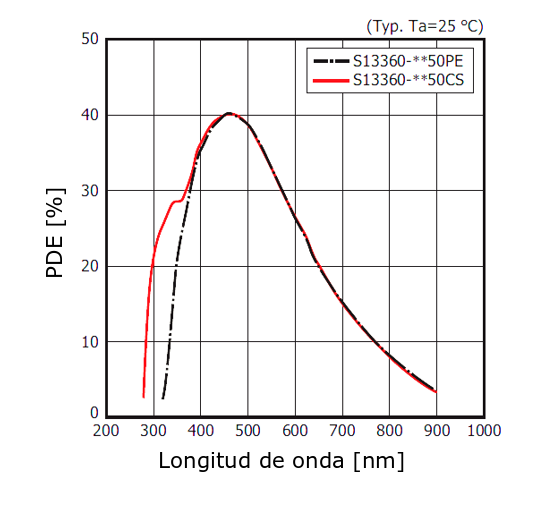
\includegraphics[width=0.5\textwidth]{Images/PDE.PNG}
    \caption{PDE en función de la longitud de onda para la serie S13360 de Hamamatsu. Adaptado de \citep{Sipm_S13360_1350CS_datasheet}.}
    \label{fig:PDE}  
  \par\end{centering}
\end{figure}

\subsubsection{Rango dinámico y linealidad.}
El máximo número de fotones que se pueden detectar simultáneamente antes de que el SiPM se sature está determinado por la cantidad de píxeles. El SiPM es lineal, si en una ventana de tiempo menor al tiempo de restablecimiento del dispositivo, el número de fotones incidentes es menor al número de píxeles. El número de píxeles activados en función del número de fotones incidentes puede ser aproximado por la siguiente expresión:
\begin{equation}
    N_{fired}=N_{pixel}\left (1-e^{-\frac{N_{photon}\cdot PDE}{N_{pixel}}}\right),
    \label{rangoDinamico}
\end{equation}
donde, $N_{fired}$ es el número de microceldas activadas, $N_{photon}$ el número de fotones incidentes y $N_{pixel}$ el número de píxeles del dispositivo \citep{Apd_Hamamatsu}.
\subsection{Ruido en SiPMs.}
El ruido en general se refiere a señales indeseadas que se superponen a una señal principal o de interés. Según \citep{tomasi} se puede clasificar el ruido en dos categorías: correlacionado y no correlacionado. El primero existe cuando hay una señal y el segundo está presente siempre, haya o no una señal.\\ \\
El ruido no correlacionado en SiPMs se denomina tasa de conteo oscuro (DCR, por sus siglas en Inglés) y es causado por electrones que generan avalanchas debido a excitación térmica proveniente de vibraciones en la red cristalina. Estos eventos son indistinguibles de los generados por un fotón, ya que generan una señal de 1 p.e. Una forma de filtrar el DRC es estableciendo un nivel de umbral superior a 1 p.e.\\ \\
Por otra parte, para el análisis de ruido en DC es conveniente medir el ruido no correlacionado como una corriente (típicamente en el orden de los nA). Esta corriente se denomina corriente oscura, debido a que se mide a la salida del SiPM cuando no están incidiendo fotones sobre este.\\ \\
El ruido correlacionado está dividido en \textit{crosstalk} y \textit{afterpulses}. El \textit{crosstalk} es causado porque los electrones que  son acelerados por el campo eléctrico en el proceso de avalancha pueden emitir fotones (infrarrojos), estos fotones viajan a las microceldas adyacentes ocasionando una avalancha secundaria. Según \citep{charct_noise} si los pulsos producidos en este proceso son simultáneos, o con un tiempo de retardo menor a 100 ps del pulso primario, son denominados \textit{crosstalk} directo y sus amplitudes son de 2 p.e, como se muestra en la fig. \ref{fig:noise}b. Por otra parte, si el retardo es mucho mayor a 100 ps se denomina  {crosstalk} retardado y su amplitud es del orden de 1 p.e, como se observa en \ref{fig:noise}c. 
\begin{figure}[h!]
\begin{centering}
  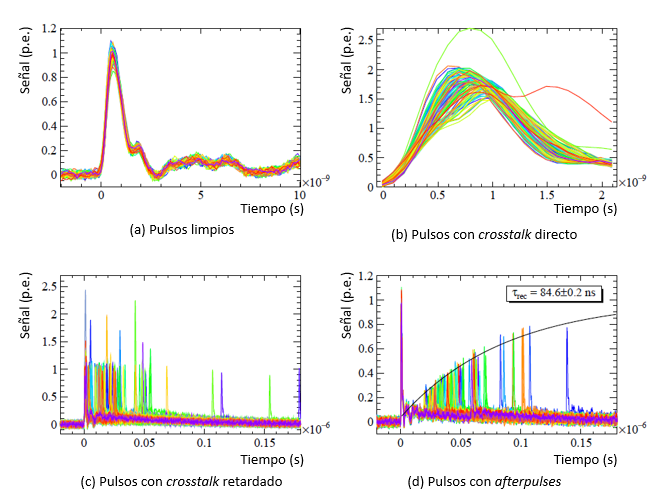
\includegraphics[width=\textwidth]{Images/Pulses_with_noise.PNG}
    \caption{Representación de amplitud y distribución temporal de pulsos sin ruido (a), con \textit{crosstalk} directo (b), \textit{crosstalk} retardado (c)  y \textit{afterpulses} (d) en un SiPM. Adaptado de \citep{charct_noise}. Se puede observar que después de  $0.1~\mu$s la frecuencia en los tipos de ruido disminuye considerablemente.}
    \label{fig:noise}  
  \par\end{centering}
\end{figure}
\\ \\
Los \textit{afterpulses} son generados durante el proceso de avalancha por portadores de carga que quedan atrapados en los niveles de energía de las impurezas  del material, pero después de un corto tiempo  (de 1 a 10 ns) adquieren la energía necesaria para saltar a la banda de conducción y generar una avalancha. Estos pulsos son del orden de 1 p.e. y pueden ser discriminados \citep{MPPC_note}. En la figura   \ref{fig:noise}d se muestra el comportamiento de los \textit{afterpulses} en función del tiempo. Finalmente, se puede concluir que para tiempos mayores a $0.1~\mu$s después del evento primario estos tipos de ruido disminuyen su probabilidad de ocurrencia considerablemente.       
\subsection{Dependencia de la temperatura.}
En los dispositivos de estado sólido la temperatura tiene una influencia importante. En los SiPM su principal efecto es sobre los coeficientes de ionización de los portadores de carga \citep{Temp_dependencia_APD}, esto genera un efecto en el voltaje de ruptura, el ruido y la ganancia.\\ \\
El voltaje de ruptura tiene una relación directamente proporcional con la temperatura, ya que al aumentarla los portadores de carga de la red cristalina sufren una dispersión  que causa una pérdida en su energía neta, esto dificulta el proceso de ionización. Para compensar esta caída en la taza de ionización es necesario aumentar el voltaje de polarización. La expresión que relaciona el voltaje de ruptura y la temperatura es la siguiente: 
\begin{equation}
    V_{BD}(T) = \frac{dV_{BD}}{dT}T+V_{BD}(0),
    \label{ruptura_eq}
\end{equation}
donde, $V_{BD}$ es el voltaje de ruptura, T es la temperatura y $V_{BD}(0)$ es el voltaje de ruptura a cero grados Celsius \citep{Charct_dep_temp}.  
\\ \\
La temperatura no tiene efectos considerables sobre el \textit{crosstalk} y \textit{afterpulses}. Sin embargo, sí los tiene sobre el DCR, ya que las vibraciones en la red cristalina generan fonones que facilitan el paso de los portadores de carga de la banda de valencia a la banda de conducción. Este aumento puede ser hasta de 50 \% por cada 10 $^\circ$C \citep{MPPC_note}.\\ \\
Según \citep{Charct_dep_temp} la probabilidad de producir pares electrón-hueco por efecto de la temperatura es:
\begin{equation}
    p(T) = CT^{3/2}e^{\left( -\frac{E_g}{2K_BT} \right)},
\end{equation}
donde, T es la temperatura absoluta, $E_g$ es la energía de la banda prohibida, $K_B$ es la contante de Boltzmann y C es una constante de proporcionalidad que depende del material y de los parámetros de la tecnología de fabricación.\\ \\
Una sugerencia de los fabricantes para mitigar los efectos de la temperatura sobre estos parámetros del SiPM, es operar los dispositivos en un entorno de temperatura controlada. Sin  embargo, para el caso  que sea inviable es necesario caracterizar los efectos de la temperatura sobre estos parámetros.      
